\documentclass{article}

\usepackage{algorithm}
\usepackage{amsfonts}
\usepackage{algpseudocode}
\usepackage{graphicx}
\usepackage{enumitem}


\title{Secure Aggregation with Global Differential Privacy for Federated Machine Learning with Malicious Clients}
\author{Olivia Roehrig  \\
	Your Company / University  \\
	\and
	Maxim Urschumzew \\
	His Company / University \\
	}

\date{\today}
% Hint: \title{what ever}, \author{who care} and \date{when ever} could stand 
% before or after the \begin{document} command 
% BUT the \maketitle command MUST come AFTER the \begin{document} command! 
\begin{document}

\maketitle


\begin{abstract}
Short introduction to subject of the paper \ldots 
\end{abstract}

\section{Introduction}
Data privacy is one of the factors motivating federated learning. A machine learning model can be trained locally on computers owned by data owners (clients), who exchange only intermediate training results (gradients), instead of the data itself, with a central server that aggregates them into a shared model~\cite{McMahan2016CommunicationEfficientLO}. While this relieves the need to collect possibly sensitive data in a central location to perform the training process, the shared model and the gradients themselves contain enough information to enable reconstruction of private information~\cite{7958568}\cite{Boenisch2021WhenTC}.

A solution to this problem is using a modified training algorithm that provides \emph{differential privacy} for the model~\cite{Abadi_2016}. The technique adds a small amount of noise to the result of each training step, calibrated in a way that makes high certainty statements about the presence of an individual point in the training dataset unlikely to be inferrable from the model.

In this document, we present an architecture that allows using federated gradient descent while providing differential privacy for the training result as well as all intermediate gradients.

Adding noise locally will require a large amount of noise and hence large utility loss to achieve privacy, so our protocol adds noise after aggregating intermediate results (\emph{global} differential privacy). To avoid revealing the non-noised aggregate to even the party adding the noise, we use the Prio protocol for \emph{secure aggregation}~\cite{prio}.

\paragraph{Threat model and privacy guarantees.}
Our system requires two non-colluding aggregation servers that can be curious but are honestly executing the protocol. All other participants, namely the clients and a server coordinating federated model updates, can be malicious. In this setting, we can guarantee anonymity (no adversary can tell which client submitted which data value) and privacy (no adversary learns anything about any honest clients' data values except the differentially private aggregate) as well as differential privacy for all information exchanged between participants as well as the final training result.

In addition, the system is robust towards data poisoning attacks by limiting the influence a single client can have on the aggregation result.

\paragraph{Related work.}
There is a variety of work on federated learning with secure aggregation and global differential privacy. Systems that provide both differ from ours by the assumed threat model:
\begin{itemize}
\item\cite{dprio} no input validation, only one out of at least two servers needs to be honest but curious, but allows only small fraction of dishonest clients
\item\cite{Stevens2021EfficientDP} no input validation, server may be malicious, but requires honest majority of clients
\item\cite{Kairouz2021TheDD} no input validation, server may be malicious, but all clients need to be honest (which is realistic when having access to trusted execution environments)
\item\cite{acorn} can do input validation, only one out of at least two servers needs to be honest but curious, but allows only small fraction of dishonest clients
\end{itemize}

\section{The \texttt{dpsa4fl} system}
The \texttt{dpsa4fl} library enables the use of the \textit{Distributed Aggregation Protocol} (DAP) for
aggregation of gradient vectors in the context of federated machine learning. It
is currently specialized to work with the janus implementation of DAP,
and the flower machine learning framework.
In practice this means that our library \texttt{dpsa4flwr} allows users of flower
to replace the native aggregation process with our alternative aggregation flow
going through a separate janus instance.

\paragraph{Architecture.}
A distributed FL system using \texttt{dpsa4fl} (figure \ref{fig:architecture}) can thus be
subdivided into two parts: the original participants of a given federated
learning scheme (comprised of a server and multiple clients), and two
janus aggregation servers executing the DAP. To differentiate the FL server from
the aggregation servers we call it the \textit{controller}.

\begin{figure}[h]
  \centering
  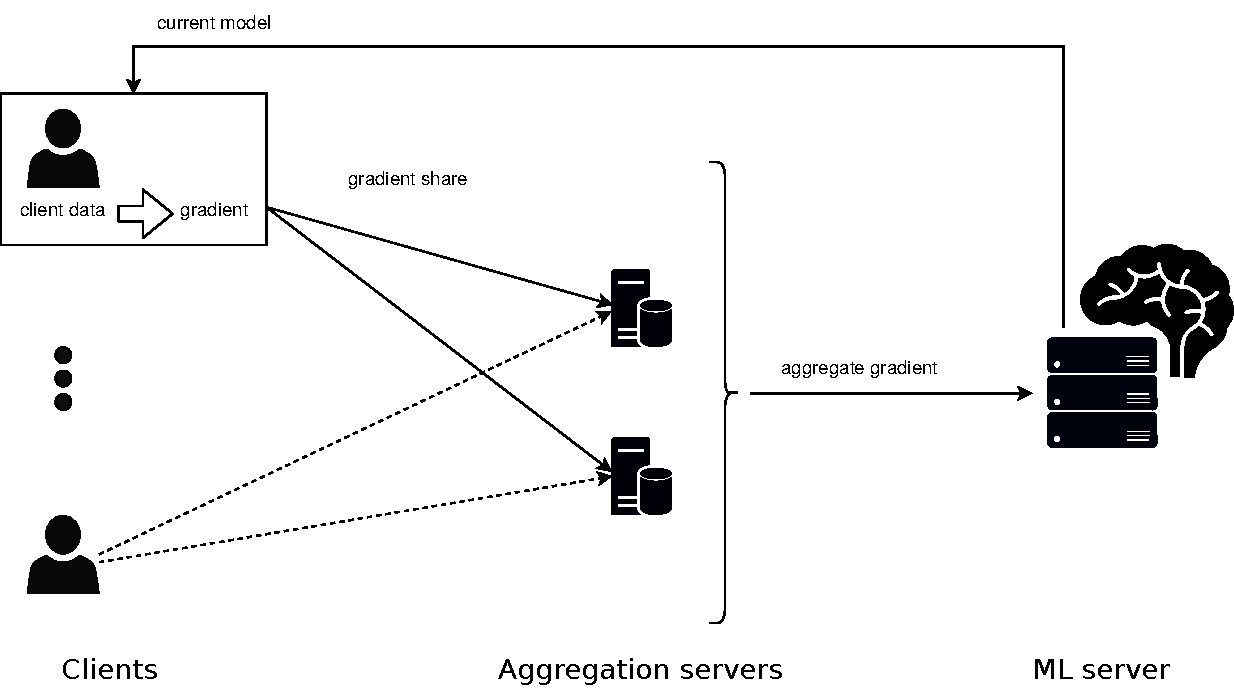
\includegraphics[width=\columnwidth]{assets/dpsa-overview-2-edit_no_explanations-2023-08-22.drawio.pdf}
  \caption{Test}
  \label{fig:architecture}
\end{figure}

The FL framework, i.e., flower, remains responsible for all functions of an FL
scheme, except for gradient aggregation. This includes broadcasting of the
current model, selecting clients for training, and applying the aggregated
gradients to the model.

The janus servers are responsible for making the aggregation of clients'
gradients secure and private. These aggregation servers do not need to be
managed by the same organization that is running the FL scheme, since they
merely provide a generic aggregation mechanism. They are intended to be long
running services which are responsible for processing aggregation jobs for
various applications concurrently. In fact, the threat model assumes that at
least one aggregation server is run by a separate organization, see section ?.

\paragraph{Intended setup.}

This means that an FL-org can delegate the additionally required infrastructure
to a ``DAP as a service''-provider, and thus get good privacy guarantees for
their users without too much organizational overhead.

\paragraph{Execution}

We describe how a single round of an FL-scheme is executed:
\begin{enumerate}[itemsep=0mm]
\item The controller selects available clients for this round and broadcasts its model to them.
\item The clients train their copy of the model on their local training data and
  compute the overall gradient vector.
\item They encode and split the gradient vector according to the prio protocol
  and submit each part to an aggregation server.
\item The aggregation servers aggregate reports from all clients, verify them,
  add noise for differential privacy and compute the sum of all gradient vectors.
\item The controller gets this gradient vector, applies it to its model, and
  begins the next round.
\end{enumerate}
It is important to note that each aggregation server receives only a ``share''
of every clients' gradient vector. It is impossible to reconstruct the original
vector from this share alone. All processing on the aggregation server, i.e.,
the verification, aggregation and noising happens in terms of its shares.
Only the subsequent combination of the resuls from both aggregation servers gives
us a plaintext value: the sum of all gradient vectors, together with noise. From
this value too it is sufficiently improbable to conclude properties of
individual clients' submissions. See section \ref{} for a more detailed analysis.

\section{Threat model}
The controller and the clients have different goals, and thus the threat model
has to be considered seperately for them. The parties running the aggregation
servers should be impartial to the learning process, but of course might deviate
from that behaviour. We consider the perspectives of the clients
and of the controller below.

\paragraph{Clients.} The clients are interested in participating in an FL-scheme
without their private information becoming known by other parties. There are two
ways this might happen:
\begin{enumerate}[itemsep=0]
\item The submitted gradient vector of a client (for a given training round) might
  become known to other parties. This would allow them to infer properties of
  the local training set.
\item Access to the trained model makes it possible to make inferences about the
  combined training set. Combination with other publicly available data can lead to
  leakage of individual clients' data.
\end{enumerate}
Our system guarantees the following: As long as at least one aggregation server
follows the protocol (i.e., is honest-but-curious), the client's data remains
private. Attack (1) is mitigated by the secure aggregation mechanism of DAP.
As long as the aggregation servers don't collude, they don't have access to
individual gradients. Attack (2) is mitigated by the fact that the sum of
gradient vectors is never revealed by itself, but only together with the noise added by
both aggregation servers. As long as at least one aggregation server adds
correctly configured noise, this makes the revealed value differentially
private. Differential privacy mitigates inference attacks (source).

In practice this means: clients can be sure that their data is safe as long as
they trust one of the aggregation servers to be honest in their execution of the
protocol. No trust in the controller is required.

\paragraph{Controller.} The controller is interested in training an ML model on
the data of the clients. Since it cannot inspect the individually submitted
gradients, this introduces the possibility of data poisoning attacks: malicious
clients can try to influence the learning process by submitting exaggerated
gradient vectors.

The DAP is designed to mitigate this sort of attack. Even though the aggregation
servers do not have access to individual plaintext gradients, they have a
protocol for verifying that each of the submitted reports is well-formed, i.e.,
has an L2-norm less than $1$. This means that while clients still can submit
``false'' data, they cannot gain unproportional leverage by doing so. Thus, data
poisoning attacks by a minority of clients are mitigated. The DAP can only
guarantee this as long as the aggregation servers do not collude with malicious
clients, as in that case it would be easy to craft submissions to fool the other
aggregation server into believing that reports are well-formed, even though they
are not.

In practice this means: the controller can be sure that it receives gradients
based on real data, as long as it trusts \textit{both} aggregation servers to
execute the protocol honestly, and a majority of clients is honest.


\section{Implementation}




\paragraph{Algorithm}

\begin{algorithm}
  \caption{Client procedure}\label{client}

  \begin{algorithmic}[1]
  \State\textbf{Input:} Training dataset $X$, loss function $\mathcal L(\theta; x)$, number of rounds $N$, fixed point encoding bit length $b$
  \State\textbf{Output:} Model $\theta$ trained on dataset $X$ for $N$ rounds

  \For{$N$}
  \State$\theta$ = retrieve current shared model from the ML server server
  \State\textbf{G} = $\frac{1}{|X|} \sum_{x\in X} \nabla\mathcal L(\theta; x)$ (model gradient average)
  \State\textbf{G} = $\textbf{G}/\mathbf{max}\{1,||\textbf{G}||_{L_2}\}$ (clip $G$ to $L_2$ norm 1)
  \State\textbf{G} = round entries towards $0$ to get $b$-bit fixed point number in $(-1, 1)$
  \State\textbf{G} = apply $p(x) = 2^{b-1}\cdot x + 2^{b-1}$ to all entries to get an integer vector
  \State send one secret share of \textbf{G} to each of the aggregation servers
  \EndFor
  \State$\theta$ = retrieve current shared model from the ML server
  \State\Return $\theta$
  \end{algorithmic}
\end{algorithm}


\begin{algorithm}
  \caption{Aggregator server procedure}\label{server}
  \begin{algorithmic}[1]
  \State \textbf{Input:} Set of clients $C$, privacy parameter $\rho$, fixed point encoding bit length $b$, finite field $F$ with order $p /geq 2^b$
  \State \textbf{Output:} Aggregate gradient, noised to be $\rho$-zero concentrated differentially private

  \State \textbf{G} = 0
  \For{all clients $\textbf{c} \in C$}
       \State \textbf{g} = retrieve gradient share from \textbf{c}
	   \State verify \textbf{g} is a share of a fixed point vector with $L_2$ norm $\leq 1$ projected to the field
	   \State \textbf{G} = \textbf{G} + \textbf{g}
  \EndFor
  \State \textbf{G} = \textbf{G} + $n$ where $n$ is drawn from the discrete Gaussian distribution $\mathcal N_\mathbb{Z}(0,\frac{2^n}{\sqrt{2\rho}})$
  \State \textbf{G} = $\textbf{G}\textnormal{ mod } p$ and map to field $F$
  \State retrieve aggregate share from other aggregation server and decrypt
  \State apply $pp(y) = 2^{1-b} \cdot y - |C|$ componentwise to obtain a float vector
  \end{algorithmic}
\end{algorithm}
\section{Privacy analysis}


\section{Utility analysis}

\bibliographystyle{plain}
\bibliography{refs}

\end{document}

